\documentclass{article}
\usepackage{float} % this is for image placement
\usepackage{blindtext}
\usepackage{fullpage}
\usepackage{graphicx} % this is so that we can have images
\graphicspath{{/images}} %path to images
\renewcommand*\contentsname{Table of Contents} % changing the default title of table of contents simply from "contents"


%here we add Abstract and acknowledgement to table of contents despite them being unnumbered sections



\title{Future of Clothing, A technological approach}
\author{Dinesh Devkota,
Maharshi Bhusal, Rajat Parajuli, Sushant Thapa}
\date{\today}

\begin{document}
\pagenumbering{roman}
\maketitle
\newpage

\section*{Acknowledgement}
\addcontentsline{toc}{section}{Abstract} % it is important to add this line after section, instead of before the \begin{document} line as doing so generates erroneous output
We would like to express our gratitude to the Department of Electronics and Computer Engineering of the Institute of Engineering, Pulchowk Campus for providing a platform for exchanging knowledge and developing one’s personal creativity. All guidance and resources provided by the college has been crucial in our vision that we present today. By assigning a major project as part of the fulfilment of the Bachelors’ Degree in Computer Engineering, the Department has helped us develop technical skills and convey the necessities in handling real life projects in the future.
We are indebted to Dr Jyoti Tandukar for being our supervisor and guiding us towards a feasible project roadmap. His guidance, experiences and expertise have been a boon for our group and crucial in developing our project to the stage it has reached. We would also like to extend our gratitude to the staff of Alternative Technology who have supported us throughout our project timeline.



\newpage

\section*{Abstract}
\addcontentsline{toc}{section}{Acknowledgement}
The project “The Future of Clothing: A Technological Approach” is a project that aims to use existing technology to improve the experience of custom designed clothing. Here, a program is written for the design of the clothes and generation of a human body model, both on the basis of user input and preference. The program further wraps the generated clothing on the body model and enables the end-user to view this model in a 3-D environment.
\newpage

\tableofcontents
\listoffigures


\newpage
\pagenumbering{arabic}
\section{Introduction}

\begin{figure}[h]
    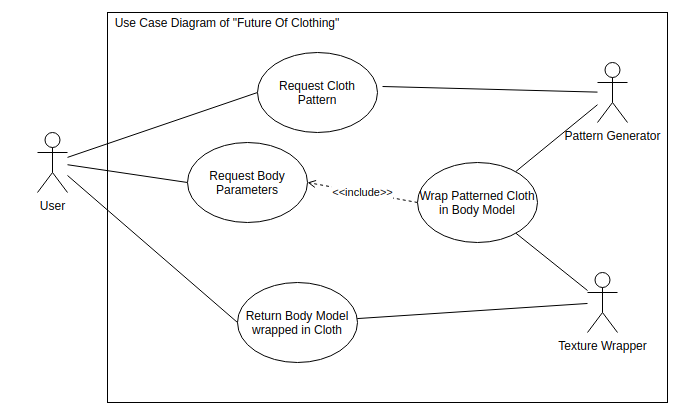
\includegraphics[scale=0.6]{images/softwareDiagrams/FinalSystemUseCase.png}
    \centering
    \caption{Use Case Diagram of the system}
    
\end{figure}
Technology in the sector of image processing has matured enough for developers to create interesting applications. With the increase in computation power, software development tools, developer communities, etc. and decrease in the cost of computer hardware it has become easier for technology creators and consumers to create and consume technology for a better quality of life.
In this project, the attention is focused towards using technology in the field of image processing and applying the said technology towards clothing. The main aim of the project is to create a system whereby a user can virtually wrap a computer generated cloth to a computer generated body of the end user. The body of the subject is based on the description provided by the users themselves. Not only is the clothing wrapped around a user defined body wireframe, but the clothing and the pattern of clothing is also user defined providing a high degree of customization from the perspective of the user. 
Patterns and designs used in the clothing can be generated by using a Generative Adversarial Network (GAN) which will synthesize new designs and patterns based on the user’s preference. Such a GAN can be trained by supplying training data based on existing design.
\newpage
\section{Literature Review}

Generating Pictures from text description has been done before quite successfully. There have also been a lot of projects in which the image was generated from parameters which can be closely related to image generation from text. Our project revolves around taking input from the user using some text and then using that information to generate images. The project also works to create a design from existing design ideas and gives the user a new unique design instantaneously, provided that the network is trained.
\subsection{Generative Adversarial Networks}
Generative Adversarial Networks (GANs) are a class of the deep neural networks which works by competing two networks namely Generative and Adversarial networks.This network was defined and introduced to the world by Ian Goodfellow in 2014 in a now legendary paper.\textbf{[ CITATION NEEDED]}. Generative Adversarial Network consist of two networks. A generative network and an Adversarial network. The generative network is a simple network which takes in gaussian noise as input and then scales and modifies the noise to create a new generated image. This generated image is the result of the GAN we need. New examples from the GANS are generated on the basis of this noise and the network. The adversarial network on the other hand is generally a classifier based on Convolutional networks. The architecture of the generative and adversarial network is not defined anywhere but generally a modified Convolutional network for adversarial and Transpose Convolutional network for generative network. However the original paper introducing GANS [ CITATION I.Goodfellow14 ] was a fully connected network for both generative and adversarial networks.\textbf{[ CITATION NEEDED]}.
The Generative and Adversarial network compete in a game to fool one another, sort of like a race. On each epochs,the generative network or generator generates new images based on the input noise  the adversarial network learns from the training data and then uses that information to verify image produced by the generative network. The real image is classified as true for the discriminator while the generated image is classified as false. Now the loss is calculated and is used to update both discriminator and the generator. If all goes well, after a few epochs the generator is able to fool the discriminator with a generated image and we get a very lifelike and real image \textbf{[citation needed]}.
 
Our architecture aims to provide a high quality geometric shapes as output. So vanilla GANs with fully connected networks cannot work as the one required as per our project. Thus we have looked into several other variation of GANs which we hope to mix in our architectures.

\subsubsection{Deep Convolutional GAN}
Deep Convolutinal GAN is a variation of GAN which is based on Deep Convolutional architecture. It uses Deep Convolutinal architecture for the dicriminator as well as Transpose Convolutional to scale the image from the noise in the generator. \cite{radford2015unsupervised}. The paper presents DCGAN as a topologically constrained variant of conditional GAN. The main benifit of usig DCGAN over classical GAN is that they are more stable to train and very useful in training unsupervised image representations. Furthermore, GANs are difficult to scale using CNN. The paper proposes to replace pooling layers with strided convolution i.e. no fully connected layers and replace it with convolutional counterparts. it further proposes to use LeakyReLU and batch normalization in all layers of discriminator while using ReLU and batch normalization in all layers of the generator(except output).
\begin{figure}[h]
    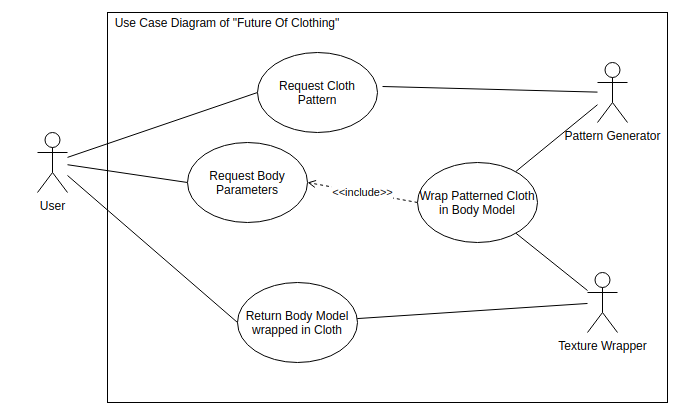
\includegraphics[scale=0.5]{images/softwareDiagrams/FinalSystemUseCase.png}
    \centering
    \caption{DCGAN architecture}    
\end{figure}

\subsubsection{StackGAN}
A very innate problem of both DCGAN and vanilla GAN is that they are unable to be scaled to higher degree. GAN is structurally an unstable architecture and it needs a lot of work to achieve momentary stability. Furthermore the complexity of any image based neural network increases exponentially with the increase in the size of the input and output. Thus the GANs which consist of large image input and output are very unstable and require a lot of processing power along with other complications in the training method. \cite{zhang} \textbf{citation needed} proposed a new system to increase the size and quality of the image produced by the GAN. In layman terms this paper proposes to stack the output of smaller GANs to the larger GANs and increase the size of the output in two times increment.
\begin{figure}[h]
    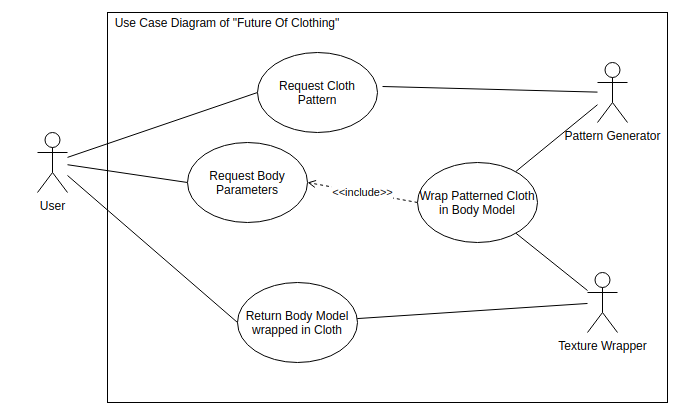
\includegraphics[scale=0.5]{images/softwareDiagrams/FinalSystemUseCase.png}
    \centering
    \caption{StackGAN architecture}    
\end{figure}


\subsubsection{StyleGAN}
GANs are very successful to provide high quality image of the natural environments and natural structures. However, vanilla and most other types of GAN fail to provide satisfactory output for a more geometric and cartoony images. StyleGAN aims to remove this problem through using a random noise in the middle of a generator architecture which will help with the sharper ends of the images.\textbf{[ CITATION NEEDED ]}. As per the website, generation of animation faces, which is similar in structure to motifs and designs are difficult to create using simple GAN architecture including the vanilla GAN architecture. The author also moves on to explain that the creation of the faces is faster and more accurate using a variant of GAN called StyleGAN.Style GAN is a Style-Based Generator Architecture for Generative Adversarial Networks is an alternative generator architecture for generative adversarial networks, borrowing from style transfer literature. The new architecture leads to an automatically learned, unsupervised separation of high-level attributes.
\begin{figure}[h]
    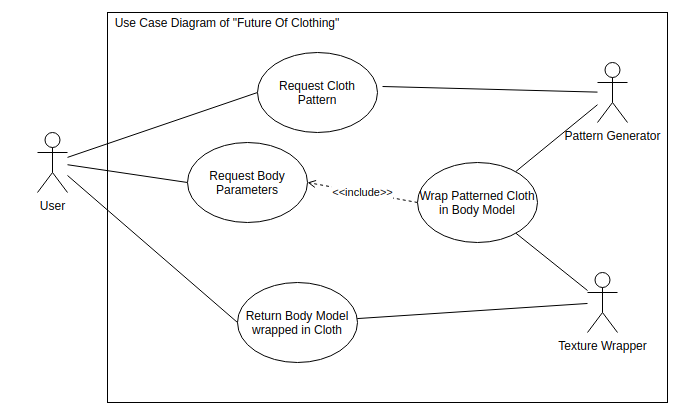
\includegraphics[scale=0.5]{images/softwareDiagrams/FinalSystemUseCase.png}
    \centering
    \caption{StyleGAN architecture}    
\end{figure}


\subsubsection{ProGAN}
GANs have always been very hard and large to train. A group of researchers of NVIDIA corporation did extensive research and have proposed a better way to train GANs. Large GANs which have very large output donot seem to scale well with complexity. Thus\textbf{citations needed}
\begin{figure}[h]
    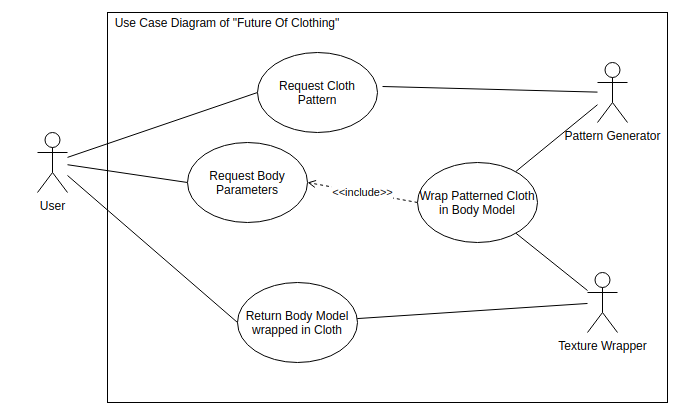
\includegraphics[scale=0.5]{images/softwareDiagrams/FinalSystemUseCase.png}
    \centering
    \caption{ProGAN architecture}    
\end{figure}

\subsubsection{WarrensteinGAN}
GANs are very difficult to train. This difficulty is in part thanks to having no good metric to provide a way to measure the success of the GANs and other generating networks. Thus the researcher are pretty much eyeballing the learning rates and other mechanism of the design. WarrensteinGAN tries to make the learning method more easy by proposing a newer and better metric to calculate the loss of the gan and provide a way to quantify their progress. WarrensteinGAN uses earth distance as a progress bar to measure the advancement of the training and provides pretty good result \textbf{citration needed}
\break

\textbf{lots of formulas here}

\subsubsection{some other gan i dont know}
it use sone way or ther to improve quality a lots \textbf{citations needd}

\subsection{3D and Depth Maps}

In 3D computer graphics and computer vision, a depth map is an image or image channel that contains information relating to the distance of the surfaces of scene objects from a viewpoint. The term is related to and may be analogous to depth buffer, Z-buffer, Z-buffering and Z-depth. The "Z" in these latter terms relates to a convention that the central axis of view of a camera is in the direction of the camera's Z axis, and not to the absolute Z axis of a scene.

Depth Maps usually follow two conventions. While both of them show the relative distance between objects in an image, one convention chooses that points closer to the focal plane are shaded lighter than those further away. The other convention does the opposite, i.e., points closer to the focal plane are shaded darker than those further away.
Although depth maps have a multitude of use cases, the one that is being explored for this project is that of automatic conversion from 2D to 3D. In computer vision single-view or multi-view images depth maps, or other types of images, are used to model 3D shapes or reconstruct them. Depth maps in general can be generated by 3D scanners or reconstructed from multiple images.
There are existing manual and semi-automatic techniques to make 3D images from 2D still images using photo editing tools like Gimp or Photoshop.
A point cloud, as the name suggests, is a collection of points in three dimensions. The most common implementation of point clouds are usually a series of coordinates, and each element in the list is treated as a point with the embedded position. Point clouds generally are not the end product. Likewise, here we further process the point cloud to generate a mesh of triangles.

We researched various algorithms like marching cube algorithm and Delaunay triangulation that generate meshes from point clouds. However, we did not have to use any of those complicated and computationally intensive algorithms as we already know the relation between the points as they were simply processed from the image.
A 3D model is comprised of many triangles and sometimes other polygons. The computational power required to render triangles increases linearly with the number of triangles in the system. However, the rate of increase of triangles with the resolution is of a parabolic nature. Using a full HD image yields over 4 million triangles. While this is theoretically feasible, it is not very practical. The framerate drop is very noticeable. Triangle reduction yields yet another problem, the mapping of the textures. Once again, we didn’t have this problem because simply lowering the resolution of the depth map gave very good results.
    
    \subsection {UV Mapping}
UV mapping is the process of mapping textures from an image into the surfaces of a 3D object. We cannot simply attach a 2D image to a 3D object we have to map every surface to a portion of the image. Since we knew where the triangles were taken from in the image, we knew exactly which portion of the image should be mapped to which surface.
There has been a lot of work done in the construction, use and manipulation of three-dimensional human body models for various purposes. Many researchers have used 3D full body scanners, 3D cameras and even the Xbox Kinect camera to capture and map human models. Similarly, a lot of research has be done to manipulate and generate new human models from the assets available by training regression functions to correlate semantically significant values \textbf{[CITATION]} or by employing the use of principal component analysis on feature curves and segment patches drawn onto the model and thus modified \textbf{[CITATION NEEDED]}. Our project will employ a mix of principal component analysis and linear regression models to generate parameters on the human body model and allow general modifications.

Among the many datasets available, the MPII Human Shape dataset \textbf{ CITATION NEEDED]} is a readily available free dataset that was used which was based on the widely used statistical body representation and learned from the CAESAR dataset, the largest commercially available scan database to date. The Polygon File Format (.ply) files obtained from the dataset formed the generic point cloud shape of the human body which was further processed in a commercially available software MeshLab \textbf{ CITATION NEEDED]} for the calculation of normal and triangulation. Further work could employ Delaunay triangulation and also spherical parameterization of 3D meshes \textbf{[]CITATION NEEDED]} for more optimized mesh construction, manipulation and also for better texture mapping.

\newpage
\section{Methodology}

    \subsection{Basic Structure of System}
        \begin{figure}[h]
            \centering
            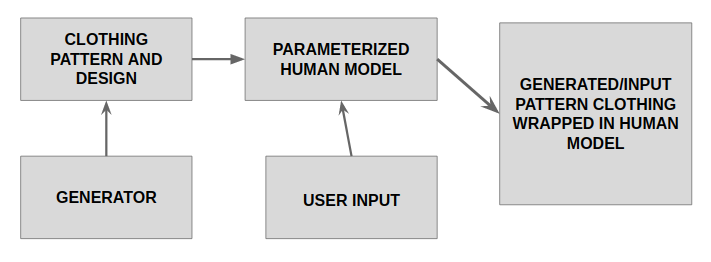
\includegraphics[scale=0.75]{images/basicArchitecture.png}
            \caption{basic architecture of system}
        \end{figure}
     
    
    \subsection{Image Synthesis using GAN}
    
    The first experiment involved generating the image of a dog. Dog images of size 64-by-64 px were generated using the GAN architecture given from the GitHub repositories \textbf{[ CITATION Mar19 \l 1033 ]} and \textbf{[ CITATION Gup19 \l 1033 ]}. The dataset used was the Stanford standard dog dataset which consisted of more than 25000 dog images and annotations in xml format. The first successful generation of the dog image was given from the kernel from \textbf{[ CITATION Deo19 \l 1033 ].}
    
    \begin{figure}[h]
        \centering
        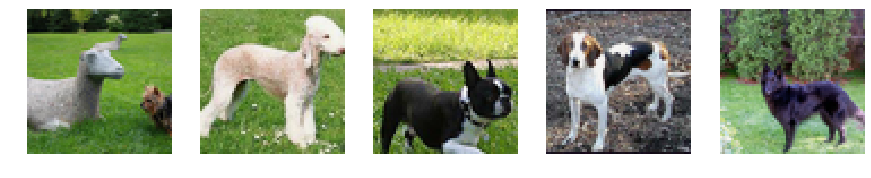
\includegraphics[scale=0.5]{images/dogGAN.png}
        \caption{Images generated by GAN}
        \label{fig:my_label}
    \end{figure}
    On the next step of our experiment we tried to generate a dandelion image from the standard flower dataset which consisted of about 1000 images of dandelion. The kernel from the dog generator was modified and used to fit our new dataset. The new generated image was also 64-by-64 px in size.
    On our next experiment we tried to make a classed generator which takes input a number and outputs the image of different classes on different numbers inputted. The kernel used was a modified version of the TensorFlow tutorial kernel which was taken from the GitHub repository \textbf{[ CITATION Lam \l 1033 ]}. However, we did not achieve much success with this kernel and thus we used a different architecture which was made by modifying the dog generator kernel.
    The latest experiment involves generation of monochrome motif designs. The motifs are converted to monochrome and then fed to the TensorFlow kernel which did not give us the expected result.
    
    \subsection{Generation of Human Body}
    
    \begin{figure}[h]
        \centering
        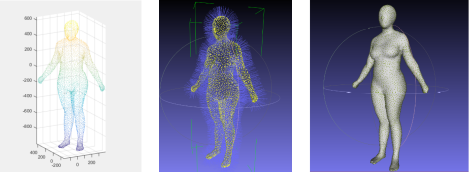
\includegraphics{images/humanModel.png}
        \caption{(Left) the extracted point cloud. (Middle) The calculated point normal in MeshLab. (Right) The mesh resulting from the screened Poisson surface reconstruction}
        \label{(Left) the extracted point cloud. (Middle) The calculated point normal in MeshLab. (Right) The mesh resulting from the screened Poisson surface reconstruction(Left) the extracted point cloud. (Middle) The calculated point normal in MeshLab. (Right) The mesh resulting from the screened Poisson surface reconstruction}
    \end{figure}
    From the MPII Human Shape dataset, the collection of 4308 models were converted from a .mat format (binary data containers that are used to include variables, functions, arrays, and other information) which contained a 6449x3 matrix of vertices in three-dimensional Cartesian coordinates into a .ply standard polygonal format for the representation of point clouds. These point clouds contained only the basic positional information of the vertices that defined the human body shape. The generated .ply files were imported into a commercially available tool called MeshLab where the point normals were generated. Then the surface was constructed using Screened Poisson Surface Construction method, both of which are available tools in the program. The model was then exported as a Wavefront object (.obj) and ready for further editing.
    
    \subsection{Depth Maps to 3D}
    
    A depth map is to distance, as a thermal image is to temperature. The closer the object, the darker it is, or lighter depending on the exact algorithm used. Just looking at a depth map does not say a lot except how far the objects are. We do not want to just know how far the object is, we want to recreate its 3D object and manipulate it or view it. An important thing to note here is that the depth map only provides us with one side of the 3d object, as evident by figure 

    \begin{figure}[H]
        \centering
        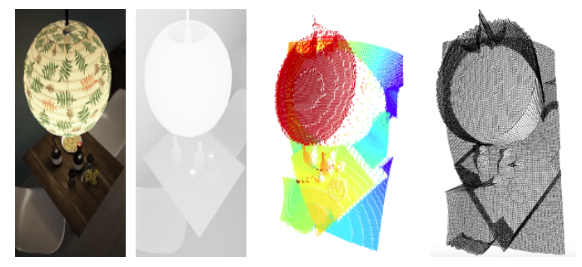
\includegraphics[width=15cm]{images/imageDMPC.png}
        \caption{Image with corresponding Depth Map,Point Cloud and Triangle Mesh}
        \label{fig:my_label}
    \end{figure}

    
    \subsubsection{Depth Map Extraction}
    
    A command line tool, called ExifTool was used to extract the depth information. It is a platform-independent Perl library plus a command-line application for reading, writing and editing meta-information in a wide variety of files. 
    \begin{figure}[H]
        \centering
        \includegraphics[scale=0.07]{images/depthMapSample.png}
        \caption{Sample image along with extracted depth map}
    
    \end{figure}
    
    
    \subsubsection{Depth Maps to Point Cloud}
    
  
  The extraction was done akin to how an actual 3d scanner works. It was assumed that the camera was in the centre of the image. A line was drawn from the camera to every pixel, then they were translated in that Line according to  their RGB values, which produces realistic renders. The illustration of the algorithm is shown in figure. It can be noticde how the darker portion of the depthmap is translated closer to the camera whereas the lighter portion of the depthmap is translated closer to the wall.
  
	\begin{figure}[H]
		\centering
		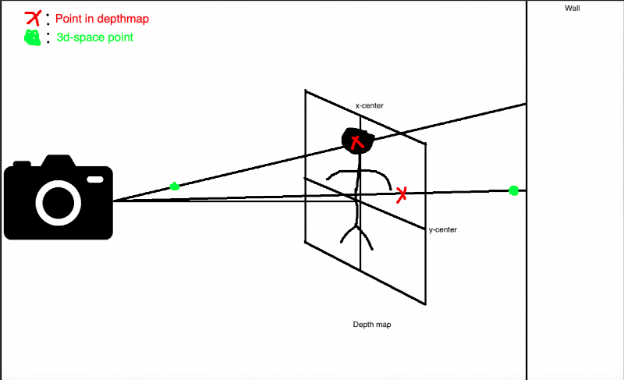
\includegraphics[width=15cm]{images/pointCloudGenerationAlgorithm.png}
		\caption{Illustration of Point Cloud Generation Algorithm}
	\end{figure}		
    
    \subsubsection{Point Cloud Triangulation}
    The surfaces must be triangulated to obtain 3D object. Normally, you can’t triangulate perfectly, as you have less information in a point cloud than a triangle mesh. In our case, we have the relation between all the pixels, and in turn all the points. This helped us achieve 100\% perfect triangulation. The result so far is a very crisp triangular mesh: A 3d object with no colors/textures. The textures need to be mapped on to the object.
\section{UV Mapping}
The process of mapping texture to a 3d object is called UV unwrapping. The process is illustrated in figure 8. When you are building an object from scratch, you also build the textures from scratch. However, we already have the textures in the colored photo. Since we also have the relationship between the surfaces and pixels, we also have the map of textures to the surfaces. The corresponding textures are now rendered in their appropriate surfaces.

\begin{figure}[H]
    \centering
    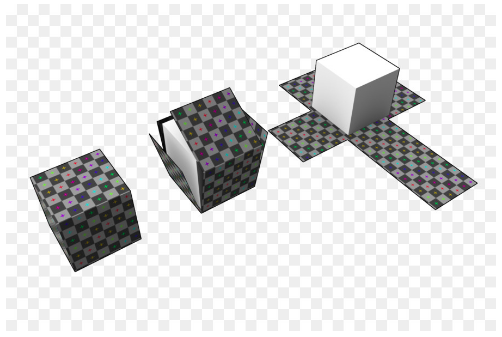
\includegraphics[width=15cm]{images/UVUnwrapping.png}
    \caption{UV unwrapping illustration}
    \label{fig:my_label}
\end{figure}


    
\newpage    
\section{Output}

\subsection{GAN outputs}

\subsubsection{Vanilla GAN with Stanford dog dataset}

\subsubsection{Vanilla GAN with Stanford Flower Dataset}

\subsubsection{Shapes with Vanilla GAN with Local Dataset}

\subsubsection{ZigZag line with DCGAN with local and synthesized dataset}

\section{Performance and Analysis}

 
\section{Conclusion}
\bibliographystyle{plain}
\bibliography{report}

\section{lines to be added}
The results of the experiments till now have been satisfactory especially in the generation of natural images. However, few problems have been noticed in the generation of high quality images and geometric images which includes shapes with precise lines and angles.

\end{document}
